\documentclass[12pt,a4paper]{report}
\usepackage[utf8]{inputenc}
\usepackage[T1]{fontenc}
\usepackage{graphicx}
\usepackage{graphics}
\usepackage{fancyhdr}
\usepackage{geometry}
\usepackage{titlesec}
\usepackage{amsmath}
\usepackage{amsfonts}
\usepackage{amssymb}
\usepackage[french]{babel}
\usepackage{shadow}
\usepackage{latexsym}
\usepackage{marvosym}
\usepackage{enumerate}
\usepackage{xcolor}

\geometry{a4paper,
  left=15mm,
  right=15mm,
  top=20mm,
  bottom=20mm
}



\usepackage{listings}
\definecolor{bgcolor}{RGB}{250,250,250}      
\definecolor{keywordcolor}{RGB}{255,140,0} 
\definecolor{commentcolor}{RGB}{50,205,50} 
\definecolor{stringcolor}{RGB}{0,90,160}    
\definecolor{numbercolor}{RGB}{255,215,0}  
\lstdefinestyle{mystyle}{
    backgroundcolor=\color{bgcolor},
    commentstyle=\color{commentcolor}\itshape,
    keywordstyle=\color{keywordcolor}\bfseries,
    numberstyle=\tiny\color{numbercolor},
    stringstyle=\color{stringcolor},
    basicstyle=\ttfamily\small\color{black},
    breakatwhitespace=false,
    breaklines=true,
    captionpos=b,
    keepspaces=true,
    numbers=left,
    numbersep=5pt,
    showspaces=false,
    showstringspaces=false,
    showtabs=false,
    tabsize=2
}
\lstset{style=mystyle}
\lstset{language=C}

\lstset{
literate=
{á}{{\'a}}1 {é}{{\'e}}1 {í}{{\'i}}1 {ó}{{\'o}}1 {ú}{{\'u}}1
{à}{{\`a}}1 {è}{{\`e}}1 {ì}{{\`i}}1 {ò}{{\`o}}1 {ù}{{\`u}}1
{€}{{\euro}}1 {ê}{{\^e}}1 {â}{{\^a}}1 {ô}{{\^o}}1
}


\begin{document}

\pagestyle{fancy}
\fancyhf{}  

\renewcommand{\headrulewidth}{1pt} 


\fancyhead[L]{\textbf{Projet : Space Invaders}}   
\fancyhead[C]{\textit{\nouppercase{\leftmark}}}  
\fancyhead[R]{\today}                              
\fancyfoot[C]{\thepage}  

\begin{titlepage}
\thispagestyle{empty}

\begin{center}

\vspace*{1cm}

% Université
{\Large \textsc{Université d'Évry Paris-Saclay}}\\[0.5cm]
\rule{0.8\textwidth}{0.5pt}\\[1.5cm]

% Titre principal
{\Huge \bfseries Space Invaders}\\[0.5cm]
{\Large \textit{Projet de programmation en langage C}}\\[2cm]


% Auteurs
{\large \textbf{RAIK Hamou \& PANN Ilfan}}\\[1.5cm]


% Formation
{\large 3\textsuperscript{ème} année de Licence en Mathématiques et Applications}\\
{\large Institut de Biologie, Génétique et Bio-informatique}\\[1.5cm]

\vspace{3cm}
% Année
{\large Année universitaire : 2025 -- 2026}

\vfill

\end{center}

\end{titlepage}


\tableofcontents
    \thispagestyle{fancy}


\newpage
\chapter{Introduction}

\section{Présentation du jeu}
    Space Invaders est un jeu vidéo iconique développé par la société japonaise Taito Corporation et sorti en 1978 sur borne d'arcade. Un jeu qui est considéré comme le premier archétype du shoot them up, où l'objectif est de détruire des vagues d'aliens au moyen d'un canon laser en se déplaçant horizontalement sur l'écran. Conçu et programmé par Tomohiro Nishikado et qui s'est inspiré  de plusieurs médias populaires de l'époque tels que Breakout ou La Guerre des mondes, il est aussi l'un des titres les plus influents de l'histoire du jeu vidéo.

\section{Objectif du projet}
Le but du projet est d’implémenter un Space Invaders, en respectant une partie des spécifications (non officielles) du jeu. Cela inclut :
\begin{itemize}
    \item  Affichage d’un menu.
    \item  Défilement vers le bas des envahisseurs, sous la forme d’une matrice de 5 lignes et 11 colonnes.
    \item  Déplacement du tank avec la souris.
    \item Gestion des tirs des envahisseurs (automatiquement) et du tank (avec l’appui sur la barre
d’espace).
    \item Gestion du score
    \item Gestion de la rapidité de défilement des éléments graphiques (envahisseurs et tirs).
    
    
\end{itemize}
On utilisera la bibliothèque \texttt{SDL2} pour la partie graphique.

\section{Compilation du code}
L’énoncé du projet impose que la compilation devra être faite avec la commande:

\begin{lstlisting}
gcc -g -O2 -Wall -Wextra -o si *.c $(pkg-config --cflags --libs sdl2)

\end{lstlisting}

Comme dans notre implémentation, nous avons ajouté une fonctionnalité sonore en utilisant la bibliothèque \texttt{SDL2\_mixer}. Donc nous avons modifié la commande de compilation  pour inclure cette dépendance :

\begin{lstlisting}
gcc -g -O2 -Wall -Wextra -o si *.c $(pkg-config --cflags --libs sdl2 SDL2_mixer)

\end{lstlisting}

Ceci nous garantit l'intégration fluide des éléments sonores.

\newpage

\chapter{Implémentation}

Le projet est constitué de plusieurs fichiers d'en-tête et source.
Dans cette section nous allons décrire les principaux aspects techniques de l’implémentation du jeu \emph{Space Invaders}.  


\section{Affichage}
\subsection{Création des pixels arts}
Dans le fichier \texttt{si\_font.c}, les éléments graphiques du jeu sont représentés à l’aide de sprites déclarés et définis sous forme de tableaux binaires de type \texttt{char}, toutes de 8 lignes avec un nombre de colonnes variable et qui sont listés ci-dessous.

    
    \begin{itemize}
    
         \item \textit{Tank}: représenté par \texttt{ si\_font\_tank[8][13]} et pour son explosion on a  \texttt{si\_font\_tank\_explode [2][8][16]} qui contient 2 sprites dans des tableaux de 8 lignes et 16 colonnes et pour le tir il est représenté par un tableau vertical et stocké dans \texttt{si\_font\_tank\_shoot[8][1]}.

    \item \textit{Invaders}:sont regroupés en trois catégories (SQUID, CRAB et OCTOPUS), chacune disposant de deux modèles pour simuler une animation simple, et sont stockés dans \texttt{ si\_font\_invaders [3][2][8][12]}, l'explosion des invaders et leurs tirs sont stockés dans \texttt{si\_font\_invader\_explode [8][13]} et \texttt{si\_font\_invader\_shoot [8][5]}

    \item \textit{Ufo}: l'ennemi mystère qui passe de temps en temps  stocké dans le tableau \texttt{si\_font\_ufo[8][16]}

    \item \textit{Les caractères alphanumériques} sont au nombre de 43 et sont stockés dans un tableau à 3 dimensions \texttt{si\_font\_alphanum[43][8][5]} 
   
   
\end{itemize}
 
    Exemple :
   \begin{center}
\begin{minipage}{0.45\textwidth}
\begin{lstlisting}
char si_font_tank[8][13]={

  {0,0,0,0,0,0,1,0,0,0,0,0,0},
  {0,0,0,0,0,1,1,1,0,0,0,0,0},
  {0,0,0,0,0,1,1,1,0,0,0,0,0},
  {0,1,1,1,1,1,1,1,1,1,1,1,0},
  {1,1,1,1,1,1,1,1,1,1,1,1,1},
  {1,1,1,1,1,1,1,1,1,1,1,1,1},
  {1,1,1,1,1,1,1,1,1,1,1,1,1},
  {1,1,1,1,1,1,1,1,1,1,1,1,1}
  
};
\end{lstlisting}
\end{minipage}%
\hfill
\begin{minipage}{0.5\textwidth}
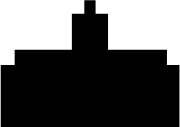
\includegraphics[width=\textwidth]{tank.png}
\end{minipage}
\end{center}

\subsection{Création d'une fenêtre graphique}
   La fenêtre est créée avec SDL. On a défini sa hauteur en fonction de la hauteur de notre écran personnel. Nous avons ensuite défini la largeur en fonction de la hauteur pour avoir le bon ratio. Ensuite une fonction SDL nous permet de récupérer les dimensions de l'écran pour pouvoir placer la fenêtre au centre 
\begin{lstlisting}

  /* Récupère les dimensions de l'écran */
  SDL_GetCurrentDisplayMode(0, &dm);
  int x = dm.w/2 -273 +3; 
  int y = g->window_height/2 -360; 
  /* Création de la fenêtre */
  g->win = SDL_CreateWindow("Space Invaders", x, y, g->window_width, g->window_height, SDL_WINDOW_SHOWN);
  if (!g->win) return NULL; 
  /* Création du rendu associé à cette fenêtre */
  g->ren= SDL_CreateRenderer(g->win, -1, SDL_RENDERER_ACCELERATED);
  if (!g->ren) return NULL;

\end{lstlisting}

\subsection{Affichage des éléments graphiques}
    Pour pouvoir afficher nos pixel arts à une taille bien visible, on parcourt la matrice d'un sprite et quand il y a un 1, on affiche le pixel comme un carré de côté 3.

\begin{lstlisting}
    void si_display_sprite(Game *g, char *data, int rows, int cols, int x, int y)
    {
      for (int w = 0; w < rows; w++) {
        for (int h = 0; h < cols; h++) {
          if (data[w * cols + h]) {
    	SDL_Rect pixel = {
    	  x + h * g->pixel_size,
    	  y + w * g->pixel_size,
    	  g->pixel_size,
    	  g->pixel_size
    	};
    	SDL_RenderFillRect(g->ren, &pixel);
          }
        }
      }
    }
\end{lstlisting}
    La fonction \texttt{si\_display\_sprite} permet ainsi d'afficher n'importe quel sprite juste en renseignant ses dimensions et ses coordonnées.
    On peux ensuite s'en servir dans une autre fonction \texttt{si\_invaders\_display} , qui affiche une vague d'ennemis en entier. 
    Les envahisseurs sont représentés par une matrice
\texttt{matrice[5][11]} dont chaque case contient :
\begin{itemize}
  \item 0 : vide (ennemi éliminé),
  \item 1,2,3 : type d'ennemi (squid / crab / octopus) utilisé pour le score et le sprite.
\end{itemize}

\begin{lstlisting}
void si_invaders_display(Game *g, int x0, int y0)
{
    char *m = si_get_matrix();

    /* Dimensions d’un sprite invader : 8 lignes x 12 colonnes */
    const int w = 12 * g->pixel_size;
    const int h = 8  * g->pixel_size;
    /* Espacement entre chacun des invaders */
    const int gap_x = 2 * g->pixel_size;
    const int gap_y = 5 * g->pixel_size;

    for (int row = 0; row < 5; ++row) {
        for (int col = 0; col < 11; ++col) {

            int v = m[row * 11 + col];
            if (v == 0) continue;
            //  1,2,3 dans la matrice d'ennemis -> type 0,1,2 pour si_invader_display
            int type = 0;
            if (v == 1)
	           type = 0;
            else if (v == 2)
	           type = 1;
            else if (v == 3)
	           type = 2;
            else continue; /* valeur inattendue */

            int x = x0 + col * (w + gap_x);
            int y = y0 + row * (h + gap_y);

            si_invader_display(g, type, g->invader_frame, x, y);
        }
    }
}
\end{lstlisting}

\vspace{1cm}
Résultat obtenu : 
\\
\begin{center}

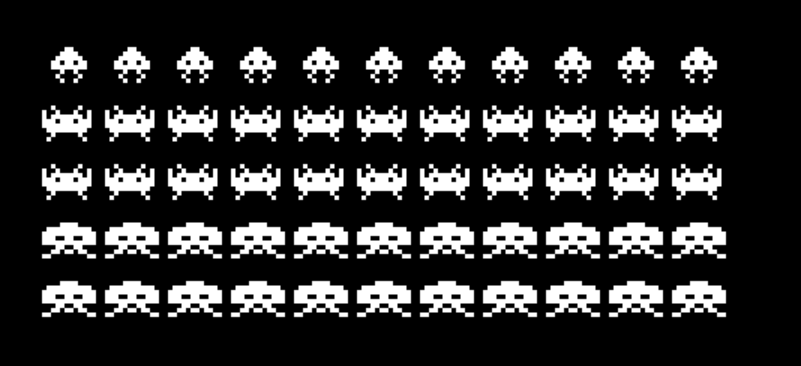
\includegraphics[scale=0.8]{invaders.png}
    
\end{center}

\vspace{1cm}
    Il y a aussi la fonction \texttt{si\_text\_display} qui permet d'écrire du texte, ici on ne passe pas par des coordonnées sur la fenêtre mais par des lignes et des colonnes. La taille de la fenêtre graphique a été découpée en 30 lignes et 26 colonnes, ses dimensions permettent d'écrire exactement 1 caractère par ligne et par colonnes.

\newpage

\begin{lstlisting}
/* Fonction qui affiche une phrase à l'écran */
void si_text_display(Game *g, const char *text, int ligne, int colonne, int spacing)
{
    /* 1. On calcule la position de départ (Haut-Gauche) */
    /* On suppose qu'une case de la grille fait 7 unités de large (5px de lettre + 2px d'espace) */
    /* Et 8 unités de haut (hauteur de la lettre) */
    int x = colonne * (7 * g->pixel_size); 
    int y = ligne   * (8 * g->pixel_size);

    /* 2. On parcourt le texte lettre par lettre */
    for (int i = 0; text[i] != '\0'; i++) 
    {
        /* On récupère l'index du caractère dans notre tableau de police */
        int index = font_index_from_char(text[i]);

        /* On affiche le sprite de la lettre */
        /* 8 = hauteur du sprite, 5 = largeur du sprite */
        si_display_sprite(g, &si_font_alphanum[index][0][0], 8, 5, x, y);

        /* 3. On déplace le curseur X vers la droite pour la prochaine lettre */
        /* Décalage = (Largeur de la lettre * taille du pixel) + espacement supplémentaire */
        x += (5 * g->pixel_size) + spacing;
    }
}
\end{lstlisting}
\vspace{0.5cm}

Ainsi pour pouvoir utiliser la fonction \texttt{si\_text\_display} , il faut d'abord définir une fonction \texttt{font\_index\_from\_char} pour accéder aux matrices associées à chaque caractère du texte à afficher.
\vspace{0.5cm}

\begin{lstlisting}
/* fonction qui à un caractère associe son index dans
   si_font_alphanum définie dans si_font.c */
int font_index_from_char(char c) 
{
  /* on convertit les minuscules en majuscules */
  if (c >= 'a' && c <= 'z')
    c = c - 'a' + 'A';
    
  if (c >= 'A' && c <= 'Z') return c - 'A';
  if (c >= '0' && c <= '9') return 26 + (c - '0');
  if (c == ' ')  return 36;
  if (c == '-')  return 37;
  if (c == '<')  return 38;
  if (c == '>')  return 39;
  if (c == '=')  return 40;
  if (c == '?')  return 41;
  if (c == '*') return 42;
  /* si on a ecrit un caractère non défini on affiche un espace */
  return 36;
}
\end{lstlisting}

On a désormais un affichage fonctionnel d'images fixes, nous permettant de facilement afficher le menu, l'écran de jeu et l'écran de fin de jeu. Rajoutons ensuite des déplacements.

\section{Déplacements}

\subsection{Déplacement du tank et de son tir }
 Le \textit{Tank} est placé en bas de l'écran et peut se déplacer uniquement en horizontal, en suivant la position horizontale de la souris, dans le cas où une partie est en cours et que le jeu n'est pas en pause.

\begin{lstlisting}
   
		 case SDL_MOUSEMOTION: //si la souris est déplacée
	      {
		//on vérifie que la partie est en cours que le jeux n'est pas en pause et que le joeur posséde au moin une vie
		if (!g->paused && g->play_game && g->si->life_1 > 0) {
		   //on met à jour la position du tanks avec la position hotizontale de la souris
		  g->si->tank.x = events.motion.x;
		  si_tank_set_position(g);// fonction qui met à jour la position du tank à l'écran
		  g->update = 1;
		}
		break;
	      }	
\end{lstlisting}

 \vspace{1cm} 
Le \textit{tir du tank} se déplace verticalement. Il est initialisé sur la ligne située au-dessus du tank et centré horizontalement par rapport à celui-ci.  
Sa position est suivie à l’aide des variables \texttt{si->tank.shoot\_x} et \texttt{si->tank.shoot\_y}, et son déplacement est géré par la fonction suivante :

   

\subsection{Déplacement des invaders et de leurs tirs}
 Les \textit{Invaders} se déplacent dans deux sens, soit de droite à gauche ou de gauche à droite jusqu'à atteindre le bord de l'écran et ensuite descendent d'une ligne et vont dans le sens opposé ceci respectivement grâce au fonctions :
 \begin{itemize}
     \item \texttt{si\_invaders\_can\_move\_left (Si *si)}
     \item \texttt{si\_invaders\_can\_move\_right (Si *si)}
 \end{itemize}    

\textbf{Exemple: \texttt{si\_invaders\_can\_move\_right (Si *si)}}
\\ Renvoie 1 si les ennemis peuvent se déplacer vers la droite, 0 sinon et met à jour la position de la matrice.

    \begin{lstlisting}
int si_invaders_can_move_right(Si *si)
{
  /*si les invaders vont à gauche on fait rien*/
    if (si->invaders.direction != 1) 
        return 0;
    int min_row, max_row, min_col, max_col;
   
    if (!invaders_alive(&min_row, &max_row, &min_col, &max_col))
        return 0;

    int inv_w = 12 * si->pixel_size;//largeur des invaders
    int gap_x = 2 * si->pixel_size;//Espacement entre les invaders
    /* colonne la plus à droite  encore vivante */
    int right_x = si->invaders.x + max_col * (inv_w + gap_x) + inv_w;

    /*si cette colonne ne dépasse pas la largeur de la fenêtre on avnce*/
    if (right_x + si->pixel_size <= si->window_width)
      {
	       si->invaders.x += si->pixel_size;//déplacement à droite  
	       return 1; 
      }
    /* on descend et on change de sens */
    si->invaders.y += 8 * si->pixel_size;// descente verticale
    si->invaders.direction = -1;// inversion du sens de déplacement 
    return 1; // mouvement effcetué
}
\end{lstlisting}

\textit{Les bombes des invaders} se déplacent aussi de manière verticale, une fois qu'on a choisi aléatoirement une colonne parmi les 11 de la matrice des ennemis grâce à la fonction,\\ \texttt{si\_invaders\_get\_column(Si *si)} on cherche l'invader le plus bas encore en vie et la bombe part en dessous de celui ci et le déplacement est géré par la fonction:

\begin{lstlisting}
    int si_invaders_bomb_can_move_down(Si *si)
{
  /* si aucun invader n'est entrain de tirer il n'y a rien à déplacer*/
  if (si->invaders.firing==0) return 0;
  
  si->invaders.bomb_y += si->pixel_size;// déplacement vertical de la bombe ennemi

  /*si la bombe sort de l'écran par le bas firing est remis à 0 */
  if(si->invaders.bomb_y >= si->window_height){
    si->invaders.firing=0;
    return 1;
  }

  /*test de collision entre le rectangle du tank et celui de la bombe*/
  if(si_tank_is_hit(si)==1)
    return 1;
  return 1;// la bombe continue sont déplacement 
}
\end{lstlisting}
    Pour finir, un minuteur est défini dans la fonction \texttt{game\_run} (qui est la boucle principale du jeu) pour faire appel à ces fonctions de déplacements. Ce minuteur permet de gérer la fréquence à laquelle on déplace les invaders, ce qui permet de contrôler la vitesse de déplacement des ennemis.

\subsection{Déplacement de l'UFO}
 L'\textit{Ufo} se déplace soit de droite à gauche ou de gauche à droite jusqu'à atteindre le bord de l'écran puis disparais ensuite. 
 Ses déplacements sont gérés, comme pour les invaders, dans la fonction \texttt{game\_run}.
 Chaque appartion de l'Ufo déclenche un cooldown de 15 secondes car c'est un ennemi qui fait des apparitions rarement. Une fois le cooldown terminé, pour qu'il fasse des apparitions aléatoires, on lui met 20\% de chance d'apparaître chaque seconde.
 
\begin{lstlisting}
	  /* APPARITION DE L'UFO */
	  Uint64 now = SDL_GetPerformanceCounter();
	  /* temps écoulé depuis le dernier test */
	  double dt = (double)(now - g->si->ufo.spawn_counter) / g->freq;

	  /* on attend 15 secondes avant d'essayer de spawn un ufo,
	     puis on tente un spawn chaque seconde
	   */
	  if (!g->si->ufo.active && now >= g->si->ufo.next_spawn_allowed && dt > 1.0) {
	    g->si->ufo.spawn_counter = now; // reset timer des tests

	    if ((rand() % 100) < 20) { // 20% de chance d'apparaitre
	      g->si->ufo.active = 1;
	      g->si->ufo.y = 35 * g->pixel_size;
	      g->si->ufo.dir = (rand() % 2) ? 1 : -1;

	      int ufo_w = 16 * g->pixel_size;
	      g->si->ufo.x = (g->si->ufo.dir == 1) ? -ufo_w : g->window_width;

	      /* on définit le prochain spawn autorisé dans 15 secondes */
	      g->si->ufo.next_spawn_allowed = now + (Uint64)(15 * g->freq);

	      g->update = 1;
	    }
	  }
\end{lstlisting}
 
L'Ufo se déplace ensuite par la même méthode que les invaders, avec un minuteur, seule sa vitesse change car il est plus rapide.



\section{Collisions}


La détection des collisions dans le jeu repose sur une modélisation simplifiée des entités graphiques à l’aide de rectangles alignés sur les axes, appeler (\textit{Axis-Aligned Bounding Boxes}).  
Chaque élément susceptible d’entrer en collision (tank, projectiles, envahisseurs) est associé à un rectangle défini par sa position à l’écran et ses dimensions.

Une collision est détectée lorsque les projections horizontales et verticales de deux rectangles se chevauchent simultanément.  

\subsection{Collisions des bombes avec le tank}
Cette collision est détectée lorsque le rectangle représentant la bombe tiré par un invader intercepte le rectangle représentant le tank.  
En cas d’impact, le tank est marqué comme détruit, une vie est retirée au joueur et un effet sonore d’explosion est déclenché.  
Le tir ennemi est ensuite supprimé afin d’éviter toute collision multiple.
La collision est  géré par la fonction suivante:
\begin{lstlisting}
    int si_tank_is_hit(Si *si)
{
  /*si les invaders ne tirent pas le tank ne peut pas être touché*/
  if(si->invaders.firing == 0) return 0;

  /*coordonées et dimensions du rectangle de la bombe des invaders*/
  int bx = si->invaders.bomb_x;
  int by = si->invaders.bomb_y;
  int bw = 5 * si->pixel_size;
  int bh = 8 * si->pixel_size;

  /*coordonnées et dimensions du rectangle du  tank*/
  int tx = si->tank.x;
  int ty = si->window_height - (16 * si->pixel_size); 
  int tw = 13 * si->pixel_size;
  int th = 8 * si->pixel_size;

  /*test de collision avec l'intersection des 2 rectangles */
  if (bx < tx + tw && bx + bw > tx && by < ty + th && by + bh > ty)
    {
      si->tank.destroyed = 1; //le tank est touché donc il est mit sur l'état de déstruction
      si->invaders.firing = 0;//arrêt du tir de l'invader
      si->sound_explode_flag = 1;// déclenchement du son de l'explosion
      return 1;
    }
  /*aucune collision détecté*/
  return 0;
}
\end{lstlisting}

\subsection{Collisions des tirs du tank avec les ennemis}


Deux fonctions gèrent les collisions entre le tir du tank et les ennemis:.


\paragraph{\texttt{si\_invader\_is\_hit(Si *si)}}  
Teste si le tir touche un invader en parcourant la matrice des ennemis et vérifie  l'intersection des rectangles correspondants.  
En cas de collision : l'invader est supprimé, le score est mis à jour, le meilleur score est éventuellement modifié et le son d'explosion est déclenché. La fonction retourne 1 si un invader est touché, 0 sinon.

\paragraph{\texttt{si\_ufo\_is\_hit(Si *si)}}  
Teste si le tir touche l'UFO. La collision est déterminée par l'intersection des rectangles du tir et de l'UFO.  
Si une intersection se produit : l'UFO est retiré, le tir arrêté, un nombre de points aléatoires (50, 100, 150 ou 300) est ajouté au score et un son d'explosion est déclenché. La fonction retourne le nombre de points obtenus si l'UFO est touché ou 0 sinon.




\section{Etats de la partie}

\subsection{Stockage des données}
    La structure \texttt{Game} centralise la fenêtre SDL, le renderer, la configuration (dimensions, taille de pixel), les compteurs de temps. 
    En plus de ce qui était attendu, nous avons rajouté certains états : pause, invader\_frame pour l'animation des ennemis, et tout une partie audio qui ajoute une musique est des effets sonores.
\begin{lstlisting}
typedef struct
{
  SDL_Window   *win;
  SDL_Renderer *ren;

  int window_width;
  int window_height;
  int pixel_size;

  int play_game;
  int paused;
  int invader_frame;
  char update;

  Si *si;

  Uint64 freq;
  Uint64 count_invaders;
  Uint64 count_shoot;

  /* Audio */
  Mix_Music *bg_music;
  Mix_Chunk *sfx_shoot;
  Mix_Chunk *sfx_explode;
  Mix_Chunk *sfx_wave;

} Game;
\end{lstlisting}

L'état du jeu (\texttt{Si}) contient les scores, vies, vague, ainsi que trois sous-structures :
\texttt{Tank}, \texttt{Invaders} et \texttt{Ufo} contenant l'état de leur nom respectifs.

\subsection{Boucle de rendu}
La fonction \texttt{game\_update} efface l'écran (fond noir), dessine les éléments (en blanc), puis appelle :
\begin{lstlisting}
SDL_RenderPresent(g->ren);
\end{lstlisting}
L'affichage est déclenché uniquement quand \texttt{g->update == 1} afin d'éviter des rendus inutiles.

\subsection{Gestion des vagues d'ennemis}
Quand \texttt{si\_matrix\_count() == 0}, on passe à la vague suivante :
\begin{itemize}
  \item incrément de \texttt{wave},
  \item réinitialisation de la matrice d'ennemis et repositionnement du bloc d'envahisseurs,
      \begin{lstlisting}
void si_reset(Si *si)
{
  /*réinitialisation des informations du jeu*/
  si->score_1 = 0;
  si->life_1 = 3;
  si->wave = 1; 
  /*initialisation du tank*/
  si->tank.x = (si->window_width / 2) - (13 * si->pixel_size) / 2;
  si->tank.firing = 0;
  si->tank.destroyed = 0;
  /*initialisation des invaders*/
  si->invaders.x = si->pixel_size;
  si->invaders.y = si->pixel_size * 60;
  si->invaders.direction = 1;
  si->invaders.firing = 0;
  /*initialisation de l'ufo*/
  si->ufo.active = 0;
  si->ufo.spawn_counter = SDL_GetPerformanceCounter();
  si->ufo.move_counter = SDL_GetPerformanceCounter();
  si->ufo.next_spawn_allowed = SDL_GetPerformanceCounter();
  /*direction de déplacement aléatoire*/
  si->ufo.dir = (rand() % 2) ? 1 : -1;

  /*réinitialisation des effet sonnores*/
  si->sound_shoot_flag = 0;
  si->sound_explode_flag = 0;
  si->sound_wave_flag = 0;
  
  /*réinitalisation de la matrice des invaders*/
  for(int j=0; j<11; j++) matrice[0][j] = 1;//SQUID
  for(int j=0; j<11; j++) matrice[1][j] = 2;//CRAB
  for(int j=0; j<11; j++) matrice[2][j] = 2;//CRAB
  for(int j=0; j<11; j++) matrice[3][j] = 3;//OCTOPUS
  for(int j=0; j<11; j++) matrice[4][j] = 3;//OCTOPUS
}
    \end{lstlisting}
    
  \item accélération via la formule de \texttt{wave\_speed}.
    \begin{lstlisting}
	  /* Accélération de la vitesse des invaders en fonction de la vague */
	double wave_speed = 0.5 - ((g->si->wave) * 0.1);
	  if (wave_speed < 0.05) wave_speed = 0.05;
    \end{lstlisting}
\end{itemize}


\subsection{Gestion du score}
Le score gagné dépend du type d'ennemi (valeur stockée dans la matrice) :
\begin{itemize}
  \item type 1 : 30 points
  \item type 2 : 20 points
  \item type 3 : 10 points
\end{itemize}
L'UFO donne un bonus aléatoire.
Le hi-score (score le plus élevé) est chargé au démarrage depuis \texttt{highscore.txt}, puis mis à jour quand
\texttt{score\_1} dépasse \texttt{score\_highest}. On réécrit alors le fichier.





\subsection{Gestion des touches}
Certaines touches ont été implémentées avec SDL pour gérer l’état global du jeu :
\begin{itemize}
  \item \texttt{Echap} ou \texttt{q} : quitter
  \item \texttt{Espace} : tirer en jeu ou relancer une partie depuis menu/game over
  \item \texttt{s} : stop / reprise du jeu
  \item \texttt{Mouvements de souris} (\texttt{SDL\_MOUSEMOTION}) : déplacer le tank horizontalement
\end{itemize}


\chapter{Les problèmes rencontrés}
\section{Ennemis se déplaçant trop rapidement}

\textbf{Explication :} Le déplacement des ennemis était beaucoup trop rapide lors de leur première implémentation, le problème ne vennait pas de la fonction qui les déplace mais de la boucle de jeu \texttt{game\_run} qui appellait la fonction de déplacement très vite. 

\textbf{Solution trouvée :}
\\
Nous avons utilisé le compteur haute-précision de SDL (\texttt{SDL\_GetPerformanceCounter}) pour mesurer le temps entre deux mises à jour, puis calculé un delta-temps (\texttt{dt\_invaders}) représentant le nombre de secondes écoulées depuis le dernier déplacement.
Ce \texttt{dt\_invaders} est ensuite comparé à une durée minimale (\texttt{wave\_speed}) :
Tant que dt\_invaders est inférieur à wave\_speed : aucun mouvement
Dès qu’il dépasse wave\_speed les ennemis se déplacent une seule fois, puis le compteur est réinitialisé.
Cela permet d’obtenir une vitesse indépendante des performances de l'ordinateur, stable peut importe la machine.
\begin{lstlisting}
    double dt_invaders = (double)(current_time - g->count_invaders) / g->freq;
    if (dt_invaders > wave_speed) 
        {
         /* ... (on gère les déplacements) */
        }
\end{lstlisting}

\section{Sortie des invaders par le bas de la fenêtre  }
\textbf{Explication :} Lors des premiers affichages, nous avons remarqué que lorsque les invaders atteignaient le bas de l’écran, ils continuaient à descendre jusqu’à sortir totalement de la fenêtre. Ils pouvaient alors s’entremêler avec le tank et passer en dessous de celui-ci. Une fois les ennemis sortis de l’écran, le jeu se retrouvait bloqué, car il n’y avait plus d’ennemis sur lesquels tirer et le joueur devras quitter et relancer une nouvelle partie.
\\
\textbf{Solution trouvée :}
Nous avons implémenter une fonction qui vérifie si le bas du groupe d'envahisseurs a atteint le haut du tank et on calcule la position du bas des envahisseurs et la compare à celle du tank.  
La fonction retourne \texttt{1} si une collision se produit et \texttt{0} sinon. Cela permet de déterminer si les envahisseurs ont progressé jusqu'à la zone défensive du joueur.

\begin{lstlisting}
int si_check_collision_bottom(Si *si)
{
    int min_row, max_row, min_col, max_col;
    /*on vérifie s'il reste des invaders non détruits et on récupère leurs limites*/
    if (!invaders_alive(&min_row, &max_row, &min_col, &max_col))
        return 0; // plus d'invaders

    int inv_h = 8 * si->pixel_size;//hauteur d'un invader
    int gap_y = 3 * si->pixel_size;// espacement vertical

    /* bas des envahisseurs */
    int invaders_bottom =
        si->invaders.y + max_row * (inv_h + gap_y) + inv_h;
    /*position du heut du tank*/
    int tank_top = si->window_height - (16 * si->pixel_size);
    
    return invaders_bottom >= tank_top;// renvoie 1 si les invaders on atteint ou dépassé le tank
}

\end{lstlisting}


\section{Matrice d'envahisseurs considérée “pleine”}
\textbf{Explication :} Les invaders font demi-tour trop tôt lorsque des colonnes sont détruites. Le calcule prends en compte toutes les colonnes de la matrice des invaders pour savoir s'ils sont arrivés au bord de l'écran, même les colonnes vides d'ennemis. Résultats :  les invaders font demi-tour trop tôt avant d'avoir atteint une extrémité de la fenêtre (gauche ou droite). 
Le même problème s'est posé aussi pour calculer si les invaders sont arrivés en bas au niveau du tank, les lignes vides d'ennemis sont prisent en compte dans le calcule des collisions. Résultats : collisions trop tôt. 
\newline 
\indent \textbf{Solution trouvée :} Création d'une nouvelle fonction qui permet de revoyer les extrémités réelles de notre matrice d'ennemis, pour pouvoir ensuite faire les tests de collisions avec les bords.
\vspace{0.5cm}
\begin{lstlisting}
static int invaders_alive(int *min_row, int *max_row, int *min_col, int *max_col)
{
    int found = 0;
    int rmin = 5, rmax = -1, cmin = 11, cmax = -1;

    for (int r = 0; r < 5; r++) {
        for (int c = 0; c < 11; c++) {
            if (matrice[r][c] != 0) {
                found = 1;
                if (r < rmin) rmin = r;
                if (r > rmax) rmax = r;
                if (c < cmin) cmin = c;
                if (c > cmax) cmax = c;
            }
        }
    }

    if (!found) return 0;
    *min_row = rmin; *max_row = rmax;
    *min_col = cmin; *max_col = cmax;
    return 1;
}
\end{lstlisting}

\chapter{Ajouts et améliorations possibles}

Malgré le fait que les instructions du projet donnent un jeu fonctionnel, nous avons fait le choix de rajouter certaines choses supplémentaires, comme la structure \texttt{Ufo }qui gère l'Ufo . De plus on a rajouté une touche pour mettre le jeu en pause en appuyant sur la touche \texttt{s}. 
Pour finir, l'ajout le plus important est celui de musiques et sons à l'aide la bibliothèque <SDL2/SDL\_mixer.h>.
\begin{lstlisting}
    /* NOUVEAU : Init Mixer (Audio) */
  if(Mix_OpenAudio(44100, MIX_DEFAULT_FORMAT, 2, 2048) < 0) {
      printf("Erreur SDL_Mixer: %s\n", Mix_GetError());
  }

  /* Chargement des sons */
  g->bg_music = Mix_LoadMUS("music.mp3");
  g->sfx_shoot = Mix_LoadWAV("shoot.wav");
  g->sfx_explode = Mix_LoadWAV("explosion.wav");
  g->sfx_wave = Mix_LoadWAV("wave.wav");

  /* Lancer la musique en boucle (-1) */
  if(g->bg_music) Mix_PlayMusic(g->bg_music, -1);
\end{lstlisting}
Trois nouveaux membres dans la structure (\texttt{Si}) nous permettent de gérer les effets sonores des tirs, de l'explosion des ennemis et de l'arrivée d'une nouvelle vague d'ennemis. 
\begin{lstlisting}
  int sound_shoot_flag;// bruit de tire
  int sound_explode_flag;//bruit d'une explosion
  int sound_wave_flag;// bruit lors d'une nouvelle vague
\end{lstlisting}
Ces variables vont jouer leur son respectif lorsqu'on met leur valeur à 1, sinon on les laisse à 0.

\vspace{0.5cm}
D'autre part, nous avons réfléchi à d'autres améliorations qui pourraient rendre le jeu encore meilleur : 
\begin{itemize}
    \item \textbf{Ajouter la possibilité d'un 2ème joueur :} Le jeu se limite à un seul joueur alors que tout est fait pour qu'on puisse jouer à deux.
    \item\textbf{Ajout de bunkers :} Le jeu original en contient, bien qu'ici ce n'était pas demandé, il serait tout de même intéressant de les implémenter.
    \item \textbf{Différents modes de jeu} L'ajout de modes supplémentaires comme le réglage du niveau de difficulté, un mode contre la montre pour détruire un maximum d'ennemis en un certain temps ou même l'ajout de nouveaux ennemis. 
    \item \textbf{Couleurs:} Les graphismes pourraient être améliorés avec une variété de couleurs pour les ennemis ou le tank.
    \item \textbf{Musique et son :} On pourrait ajouter davantage de sons et de musiques. 
    
\end{itemize}






\chapter{Sources}

\begin{enumerate}

    
  \item \textbf{Police d’écriture Space Invaders} :  

  
  \url{https://fontstruct.com/fontstructions/show/2454471/nishikado-extra}

  \item \textbf{Musique de fond} :  
  \url{https://www.youtube.com/watch?v=ITIFiLDpttw}

  \item \textbf{Son du tir du tank} :  
  \url{https://youtu.be/Dav5kn_8BmY?si=iRGuS3WsRYhsMXjf}

  \item \textbf{Son d’explosion (tank et ennemis)} :  
  8\textsuperscript{e} son de la vidéo suivante : 
  \\
  \url{https://www.youtube.com/watch?v=EA4h8l2zZ1g&t=7s}

  \item \textbf{Son de nouvelle vague d’ennemis} :  
  \url{https://youtu.be/6ga4IICXyCE?si=vWYL3BCCtvF9lspG}

  \item \textbf{Articles sur l’utilisation de l’audio avec SDL} :
  \begin{itemize}
    \item \url{https://wiki.libsdl.org/SDL2_mixer/Mix_OpenAudio}
    \item \url{https://loka.developpez.com/tutoriel/sdl/sons/}
  \end{itemize}
  \end{enumerate}
\end{document}